\documentclass{beamer}

\usepackage[T2A]{fontenc}
\usepackage[utf8]{inputenc}
\usepackage[russian]{babel}


\hypersetup {
    unicode = true
}

\usetheme{Madrid}
\usecolortheme{whale}

\title[Инструментальная среда]
{Инструментальная среда для анализа программных систем}
\author[А.М. Полоцев]{
    А.М. Полоцев гр. 63501/13\\
    Руководитель: Ицыксон В.М.\\
    Аттестация №2
}
\date[20.12.2013]{}

\begin{document}

\frame{\titlepage}

\begin{frame}
\frametitle{Разработка инструментального средства}

\begin{itemize}
    \item Цели
        \begin{itemize}
            \item Автоматизация анализа
            \item Визуализация свойств
        \end{itemize}
    \item Требования
        \begin{itemize}
            \item Поддержка анализа объектно-ориентированных языков
            \item Извлечение различных моделей анализируемой системы
            \item Встроенные средства отображения
            \item Модульная расширяемая структура
            \item Экспорт разных артефактов системы во внешние отчеты
            \item Предоставление API к разработанным методам анализа
        \end{itemize}
\end{itemize}
\end{frame}

\begin{frame}
\frametitle{Архитектура инструментального средства}

\begin{figure}[h!]
    \begin{center}
        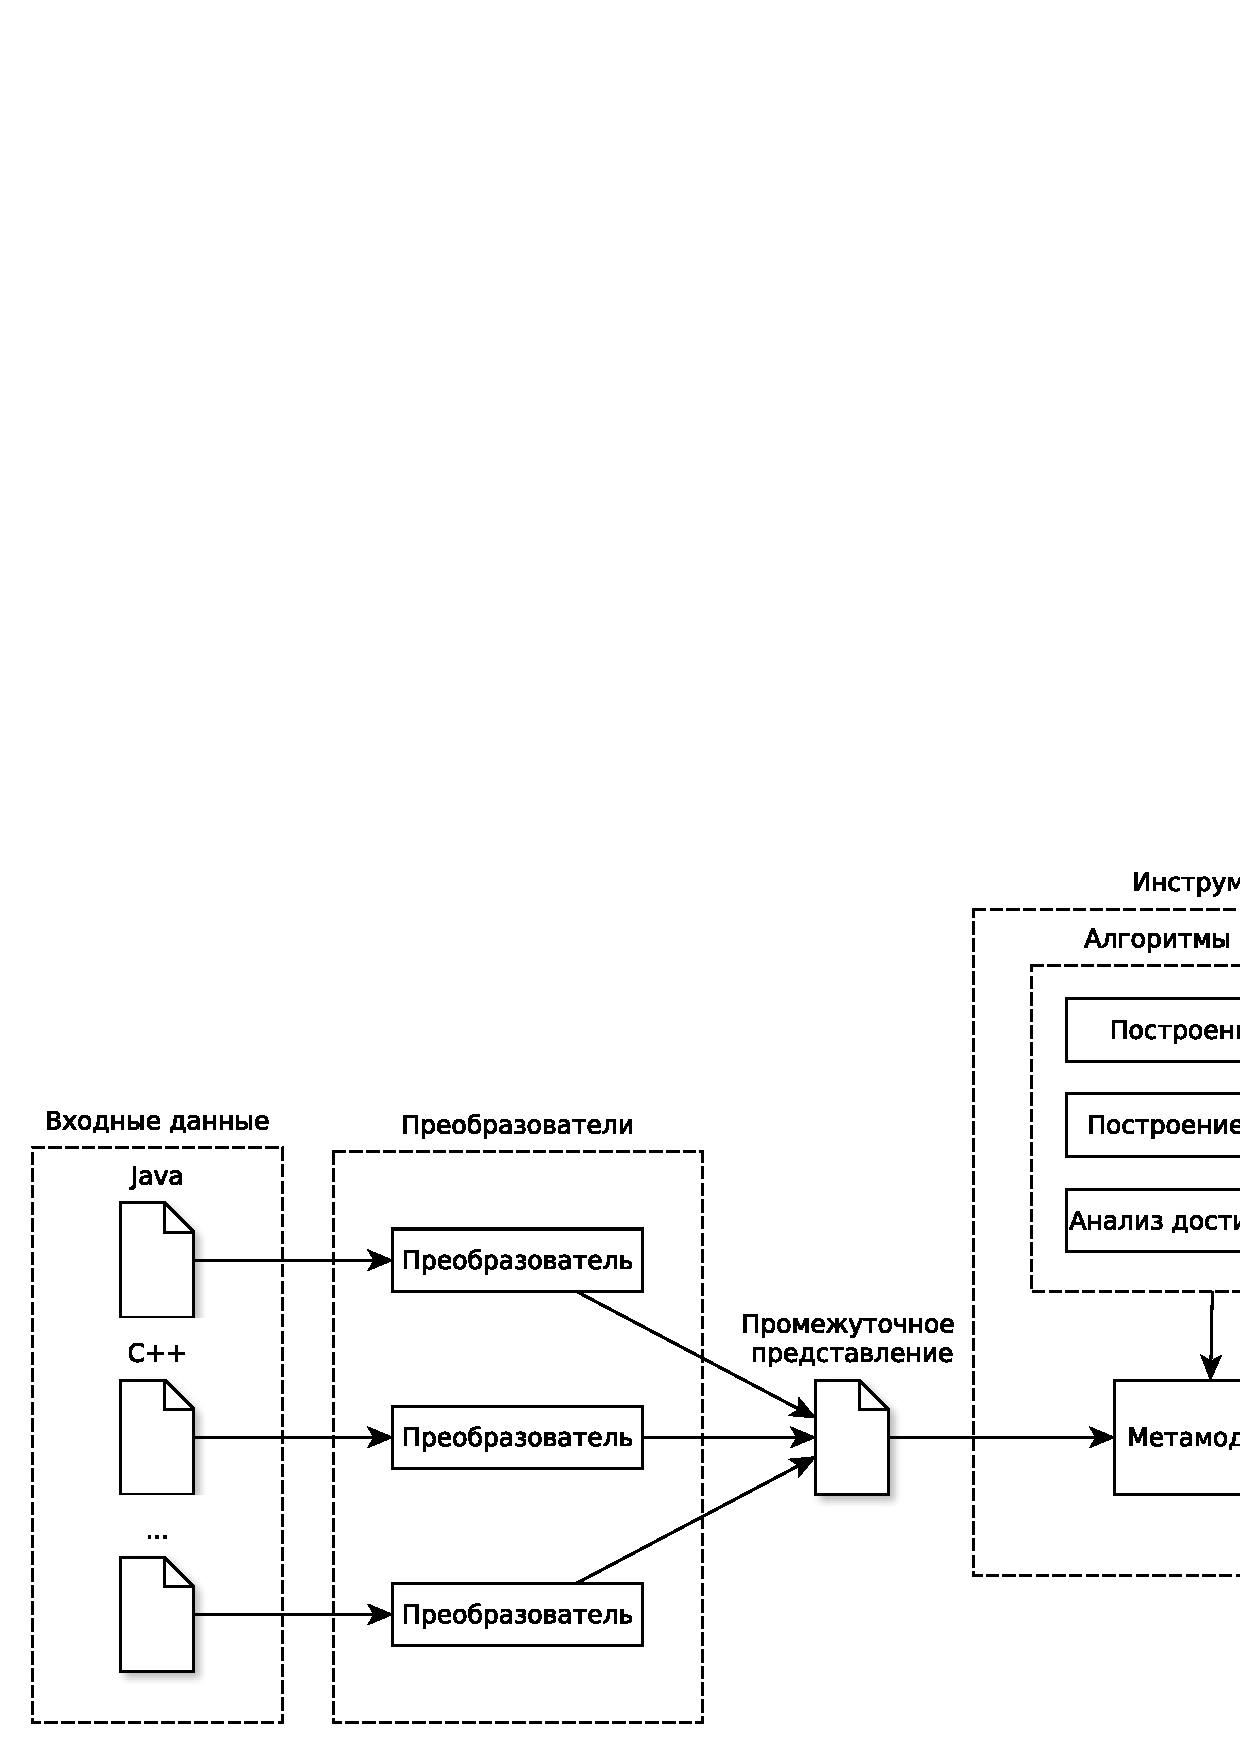
\includegraphics[width=\textwidth]{img/architecture.png}
    \end{center}
\end{figure}
\end{frame}

\begin{frame}
\frametitle{Разработка}

\begin{itemize}
    \item Разработка метамодели
        \begin{itemize}
            \item Стандарт MOF (Meta Object Facility)
        \end{itemize}
    \item Выбор промежуточного представления
        \begin{itemize}
            \item XMI (XML Metadata Interchange)
        \end{itemize}
    \item Разработка преобразователей
        \begin{figure}[h!]
            \begin{center}
                \includegraphics[width=0.9\textwidth]{img/parser_architecture.png}
            \end{center}
        \end{figure}
\end{itemize}

\end{frame}

\begin{frame}
\frametitle{Направления дальнейшей разработки}

\begin{itemize}
    \item Реализация преобразователя для языка Java
    \item Разработка методов трансформации и алгоритмов над метамоделью
    \item Разработка графического интерфейса
    \item Разработка библиотеки моделей
\end{itemize}
\end{frame}

\begin{frame}{План работы}
    \begin{itemize}
        \item[\checkmark] формулировка требований к среде
        \item[\checkmark] анализ существующих решений
        \item[\checkmark] постановка задачи магистерского исследования
        \item[\checkmark] анализ требований к среде
        \item[\checkmark] проектирование архитектуры среды
        \item проектирование API среды
        \item реализация
        \item тестирование
        \item написание пояснительной записки
    \end{itemize}
\end{frame}

\begin{frame}
\frametitle{Спасибо за внимание}
\center{\resizebox{60pt}{80pt}{?}}
\end{frame}

\end{document}
